

\section{Overlaps between structural and logical dependencies}
\label{sec:overlaps}

A logical dependency can be also a structural dependency and vice-versa, so studying the overlapping between logical and structural dependencies while filtering is important since the intention is to introduce those logical dependencies among with structural dependencies in architectural reconstruction systems. Current studies have shown a relatively small percentage of overlapping between them with and without any kind of filtering \cite{DBLP:journals/jss/AjienkaC17}. This means that a lot of non related entities update together in the versioning system, the goal here is to establish the factors that determine such a small percentage of overlapping \cite{enase19}.

Since we are first extracting co-changing pairs and only after various filters we call the remaining co-changing pairs logically dependent, we will be studying the overlapping between the remaining co-changing pairs after each filtering stage and the structural dependencies. 
For each system, we extracted the structural dependencies and the co-changing pairs and determined the overlap between the two dependencies sets, in various experimental conditions. 

One variable experimental condition is whether changes located in comments contribute towards logical dependencies. This condition distinguishes between two different cases: 
\begin{itemize}
	\item with comments: a change in source code files is counted as a co-changing pair, even if the change is inside comments in all files
	\item without comments: commits that changed source code files only by editing comments are ignored
\end{itemize}

In all cases, we varied the following threshold values: 
 \begin{itemize}
	\item commit size ($cs$): the maximum size of commit transactions which are accepted to generate co-changes. The values for this threshold were 5, 10, 20 and no threshold (infinity).  
	\item number of occurrences ($occ$): the minimum number of repeated occurrences for a co-change to be counted as logical dependency. The values for this threshold were 1, 2, 3 and 4.  
\end{itemize}

The six tables below present the synthesis of our experiments. 
We have computed the following  values:
\begin{itemize}
	\item the mean ratio of the number of co-changes to the number of structural dependencies (SD)
   	\item the mean percentage of structural dependencies that are also co-changes (calculated from the number of overlaps divided to the number of structural dependencies)	
	\item the mean percentage of co-changes that are also structural dependencies (calculated from the number of overlaps divided to the number of co-changes)
\end{itemize}

In all the six tables, \ref{tab:ratio:comm}, \ref{tab:ratio:nocomm}, \ref{tab:percSD:comm}, \ref{tab:percSD:nocomm},
\ref{tab:percLD:comm}, \ref{tab:percLD:nocomm} we have on columns the values used for the commit size $cs$, while on rows we have the values for the number of occurrences threshold $occ$. The tables contain median values obtained for experiments done under all combinations of the two threshold values, on all test systems. In all tables, the upper right corner corresponds to the most relaxed filtering conditions, while the lower left corner corresponds to the most restrictive filtering conditions.

\begin{table}[!h]
%% increase table row spacing, adjust to taste
\renewcommand{\arraystretch}{1}
\caption{Ratio of number of co-changes to number of SD, case with comments}
\label{tab:ratio:comm}
\centering

\begin{tabular}{|c|c|c|c|c|}
\hline
	      &	$cs\leq 5$	&	$cs\leq 10$	&	$cs\leq 20$	&	$cs<\infty$	\\
\hline
$occ\geq 1$	&	3,39	&	5,67	&	9,00	&	80,31	\\
$occ\geq 2$	&	2,24	&	3,47	&	5,02	&	60,14	\\
$occ\geq 3$	&	1,04	&	2,53	&	3,52	&	44,68	\\
$occ\geq 4$	&	0,90	&	2,16	&	2,88	&	33,47	\\
\hline
\end{tabular}
\end{table}

\begin{table}[!h]
%% increase table row spacing, adjust to taste
\renewcommand{\arraystretch}{1}
\caption{Ratio of number of co-changes to number of SD, case without comments}
\label{tab:ratio:nocomm}
\centering

\begin{tabular}{|c|c|c|c|c|}
\hline
	      &	$cs\leq 5$	&	$cs\leq 10$	&	$cs\leq 20$	&	$cs< \infty$	\\
\hline
$occ\geq 1$	&	3,24	&	5,33	&	7,90	&	67,16	\\
$occ\geq 2$	&	1,35	&	3,27	&	4,72	&	47,39	\\
$occ\geq 3$	&	1,00	&	1,67	&	2,49	&	32,39	\\
$occ\geq 4$	&	0,43	&	1,26	&	1,93	&	22,15	\\
\hline
\end{tabular}
\end{table}

\begin{table}[!h]
%% increase table row spacing, adjust to taste
\renewcommand{\arraystretch}{1}
\caption{Percentage of SD that are also co-changes, case with comments}
\label{tab:percSD:comm}
\centering

\begin{tabular}{|c|c|c|c|c|}
\hline
	      &	$cs\leq 5$	&	$cs\leq 10$	&	$cs\leq 20$	&	$cs< \infty$	\\
\hline
$occ\geq 1$	&	19,75	&	29,86	&	39,29	&	76,59	\\
$occ\geq 2$	&	12,50	&	20,20	&	27,68	&	66,11	\\
$occ\geq 3$	&	8,49	&	14,22	&	19,94	&	55,99	\\
$occ\geq 4$	&	6,58	&	10,95	&	15,76	&	47,12	\\
\hline
\end{tabular}
\end{table}

\begin{table}[!h]
%% increase table row spacing, adjust to taste
\renewcommand{\arraystretch}{1}
\caption{Percentage of SD that are also co-changes, case without comments}
\label{tab:percSD:nocomm}
\centering

\begin{tabular}{|c|c|c|c|c|}
\hline
	      &	$cs\leq 5$	&	$cs\leq 10$	&	$cs\leq 20$	&	$cs< \infty$	\\
\hline
$occ\geq 1$	&	18,88	&	28,47	&	37,44	&	71,12	\\
$occ\geq 2$	&	11,87	&	19,03	&	25,93	&	59,58	\\
$occ\geq 3$	&	8,00	&	13,09	&	18,15	&	48,65	\\
$occ\geq 4$	&	5,85	&	9,94	&	14,27	&	39,07	\\
\hline
\end{tabular}
\end{table}

\begin{table}[!h]
%% increase table row spacing, adjust to taste
\renewcommand{\arraystretch}{1}
\caption{Percentage of co-changes that are also SD, case with comments}
\label{tab:percLD:comm}
\centering

\begin{tabular}{|c|c|c|c|c|}
\hline
	      &	$cs\leq 5$	&	$cs\leq 10$	&	$cs\leq 20$	&	$cs< \infty$	\\
\hline
$occ\geq 1$	&	12,02	&	8,86	&	6,72	&	1,79	\\
$occ\geq 2$	&	15,05	&	11,71	&	9,38	&	2,21	\\
$occ\geq 3$	&	17,45	&	13,97	&	11,57	&	2,86	\\
$occ\geq 4$	&	18,96	&	15,28	&	12,94	&	3,67	\\
\hline
\end{tabular}
\end{table}

\begin{table}[!h]
%% increase table row spacing, adjust to taste
\renewcommand{\arraystretch}{1}
\caption{Percentage of co-changes that are also SD, case without comments}
\label{tab:percLD:nocomm}
\centering
\begin{tabular}{|c|c|c|c|c|}
\hline
	      &	$cs\leq 5$	&	$cs\leq 10$	&	$cs\leq 20$	&	$cs< \infty$	\\
\hline
$occ\geq 1$	&	12,05	&	9,02	&	6,98	&	1,93	\\
$occ\geq 2$	&	15,08	&	12,03	&	9,66	&	2,42	\\
$occ\geq 3$	&	17,78	&	14,37	&	12,24	&	3,28	\\
$occ\geq 4$	&	19,22	&	15,59	&	13,30	&	4,21	\\
\hline
\end{tabular}
\end{table}



\begin{table}[!h]
\renewcommand{\arraystretch}{1}
\caption{Percentage of SD that are also co-changing pairs after connection strength filtering. }
\label{tab:percSDstrength}
\centering
\scalebox{0.8}{
\begin{tabular}{|c|cccccccccc|c|}
\hline
Condition &	$\geq10\%$	&	$\geq20\%$		&	$\geq30\%$		&	$\geq40\%$		&	$\geq50\%$		&	$\geq60\%$		&	$\geq70\%$		&	$\geq80\%$		&	$\geq90\%$		&	$\geq100\%$	 \\
\hline
							
factor A and factor B	&	11.20	&	6.80		&	4.44	&	3.25	&	2.58	&	1.74		&	1.16	&	0.57	&	0.35	&	0.33	\\
factor A or factor B	&	15.94	&	11.02	&	7.56	&	5.59		&	4.52	&	2.90	&	2.00	&	1.33	&	1.04	&	1.02	\\
								
\hline
\end{tabular}
}
\end{table}

\begin{table}[!h]
\renewcommand{\arraystretch}{1}
\caption{Percentage of co-changing pairs that are SD after connection strength filtering. }
\label{tab:percLDtrength}
\centering
\scalebox{0.8}{
\begin{tabular}{|c|cccccccccc|c|}
\hline
Condition &	$\geq10\%$	&	$\geq20\%$		&	$\geq30\%$		&	$\geq40\%$		&	$\geq50\%$		&	$\geq60\%$		&	$\geq70\%$		&	$\geq80\%$		&	$\geq90\%$		&	$\geq100\%$	 \\
\hline
factor A and factor B	&	10.95	&	20.61	&	23.73	&	26.75	&	28.57	&	33.31	&	33.43	&	38.34	&	42.52	&	39.41	\\
factor A or factor B		&	12.19	&   16.85	&	19.41	&	20.70	&	21.63	&	22.84	&	21.86	&	23.08	&	24.00	&	22.73	\\						

\hline
\end{tabular}
}
\end{table}

In order to assess the influence of comments, we compare pairwise Tables \ref{tab:ratio:comm} and \ref{tab:ratio:nocomm},  
Tables \ref{tab:percSD:comm} and \ref{tab:percSD:nocomm} and Tables \ref{tab:percLD:comm} and \ref{tab:percLD:nocomm}. 
We observe that, although there are some differences between pairs of measurements done in similar conditions with and without comments, the differences are not significant.

On the other hand, the overlap between structural and co-changes is given by the number of pairs of classes that have both structural and co-change dependencies. We evaluate this overlap as a percentage relative to the number of structural dependencies in Tables \ref{tab:percSD:comm},\ref{tab:percSD:nocomm} and \ref{tab:percSDstrength}, respectively as a percentage relative to the number of co-changes in Tables \ref{tab:percLD:comm},\ref{tab:percLD:nocomm}, \ref{tab:percLDtrength}.

A first observation from Tables \ref{tab:percSD:comm}, \ref{tab:percSD:nocomm}, and \ref{tab:percSDstrength} is that not all pairs of classes with structural dependencies co-change. The biggest value for the percentage of structural dependencies that are also co-changes is 76.5\% obtained in the case when no filterings are done.

From Tables \ref{tab:percLD:comm}, \ref{tab:percLD:nocomm}, and \ref{tab:percLDtrength} we notice that the percentage of co-changes which are also structural is always low to very low. This means that most co-changes are recorded between classes that have no structural dependencies to each other \cite{enase19}.   



\chapter{Combining Structural and Logical Dependencies}
\label{sec:combining}

Software clustering relies on various dependencies to identify relationships between software entities. Structural dependencies have been mostly used due to their reliability \cite{SoraSem13}. However, recent research has started incorporating other types of dependencies besides structural dependencies \cite{lexical-dep}, \cite{b14}, \cite{b18}. This section will present an overview of structural and logical dependencies, focusing on how they are extracted.

\section{Structural Dependencies Weights}

Structural dependencies are important for understanding the architecture of a software system because they reveal how different modules interact at the code level. In our research, we extract structural dependencies using a tool from our previous work \cite{b4}. This tool analyzes the source code to identify various relationships between software entities and exports them in CSV format.

Structural dependencies do not all have the same level of influence on a software system’s architecture and behavior. For instance, the relationship between a variable and the class that uses it is not the same as the relationship between a class and the interface it implements. To reflect these differences, we assign different weights to each type of dependency.

The dependency types and weights were previously defined in related works on clustering \cite{SoraConti}, \cite{Finding-key-classes}.

Table \ref{tab:structural_weights} shows the weights assigned to different categories of structural dependencies, as proposed in previous works.

\begin{table}[htbp]
\centering
\begin{tabular}{|c|l|}
\hline
\textbf{Weight} & \textbf{Dependency types} \\
\hline
4 & Interface realization \\
3 & Inheritance, parameter, return type, field, cast, type binding \\
2 & Method call, field access, instantiation \\
1 & Local variable \\
\hline
\end{tabular}
\caption{Weights assigned to different structural dependency types. \cite{Finding-key-classes}}
\label{tab:structural_weights}
\end{table}

The weights are assigned based on the following considerations:

\textit{Weight 4 – Interface Realization:} Assigned the highest weight because it signifies a strong architectural relationship. Implementing an interface means classes are expected to provide specific functionalities.

\textit{Weight 3 – Inheritance, Parameter, Return Type, Field, Cast, Type Binding:} These dependencies represent significant connections between entities. They include inheritance relationships and shared data or types, which affect the behavior and properties of entities.

\textit{Weight 2 – Method Call, Field Access, Instantiation:} These indicate interactions between classes but are less impactful than higher weights. They involve using methods or fields of other classes or creating instances. When a method call, field access, or instantiation occurs multiple times between the same pair of entities, the weight is multiplied by the number of occurrences. For example, if Class A calls a method in Class B three times, the assigned weight would be 6 (weight 2 multiplied by 3).

\textit{Weight 1 – Local Variable:} Given the lowest weight, local variables are the most basic level of interaction.



\section{Logical Dependencies Weights}
\label{subsec:ld}

We refer to logical dependencies as the filtered co-changes between software entities. A co-change occurs when two or more software entities are modified together during the same commit in the version control system. Co-changes indicate that these entities are likely directly or indirectly related or dependent on each other.

Co-changes are associated with a degree of uncertainty. Compared to structural dependencies, where a dependency is certain, co-changes are less reliable. For example, if the system was migrated from one version control system to another, the first commit will include all the entities from the system at that point in time. Should we consider all these entities related to one another in this case? This would introduce false dependencies and reduce the likelihood of achieving accurate results when combining them with more reliable types of dependencies.

Even if we address the issue of the first commit, a developer can still resolve multiple unrelated issues in the same commit (even though development processes do not recommend this).

To solve this problem, in our previous works, we refined some filtering methods to ensure that the co-changes that remain after filtering are more reliable and suitable for use with other dependencies or individually \cite{b4}, \cite{DepSACI}, \cite{enase19}. Based on our previous results, the filters we decided to use further in our research are the commit size filter and the strength filter. Both filters are used together, and the result is the set of logical dependencies that we use to generate software clusters.







\subsubsection{Filter Application Process}

Fig. \ref{fig:filtering} illustrates the overall filter application process. We begin by extracting all co-changes from the versioning system, and the first filter applied is the commit size filter. The commit size filter has a strict threshold of 20 files, meaning that any co-changes from commits involving more than 20 files are filtered out.

The co-changes that remain after applying the commit size filter are then processed using the strength filter. The strength filter uses multiple thresholds, precisely 10 different thresholds. We start with a threshold of 10 and increment it by 10 until we reach a maximum value of 100. We do not use a fixed threshold to assess how different strength thresholds affect our cluster generation.

\begin{figure}[t!]
  \centering
  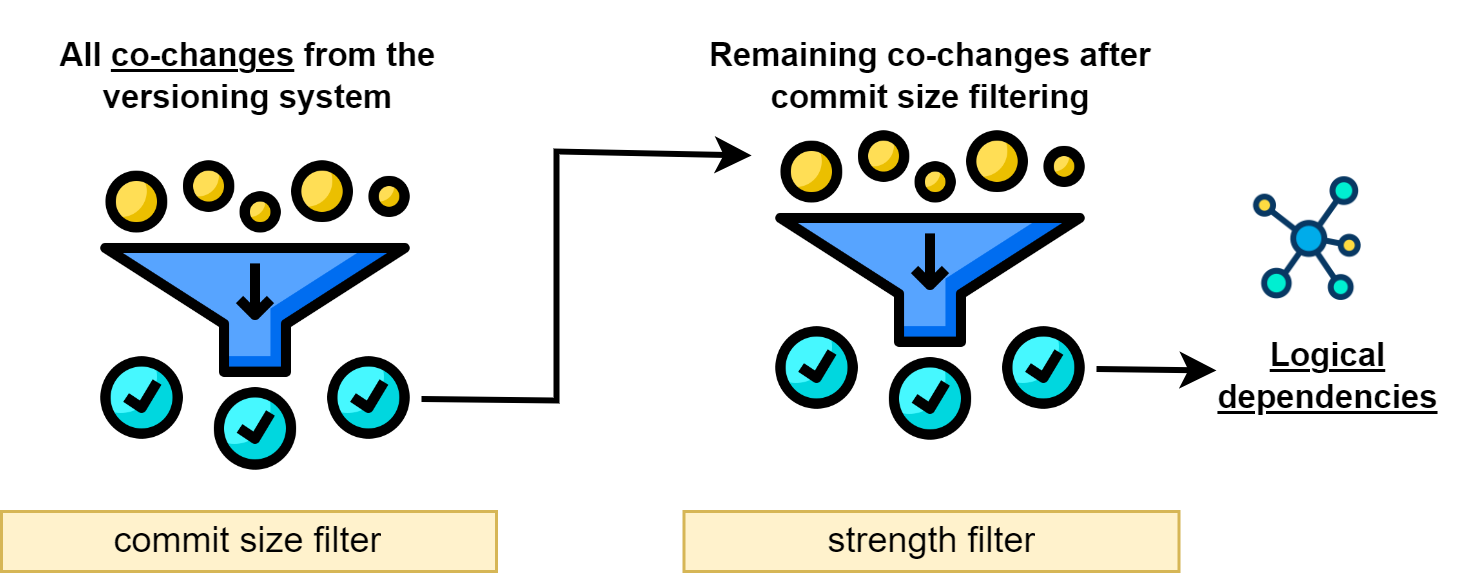
\includegraphics[width=\columnwidth]{filtering.png}
  \caption{Filter application process}
  \label{fig:filtering}
\end{figure}

\subsubsection{Dependency Extraction and Filtering Tool}

To extract and filter the co-changes, we used a previously developed tool \cite{b4}. This tool takes the GitHub repository address and the threshold values for commit and strength filters as input. The tool clones the repository, downloads all commit diffs starting from the first commit, examines all files changed in each commit to identify which entities have changed in those files, and creates undirected co-change dependencies between all changed entities within a commit.

The commit size filter is applied to these undirected co-change dependencies since the metric value for $(A \rightarrow B)$ is the same as for $(B \rightarrow A)$. For the strength filter, each co-change dependency is converted into a directed co-change dependency, so for each $(A \rightarrow B)$ dependency, we have both $(A \rightarrow B)$ and $(B \rightarrow A)$. This conversion is necessary because, as mentioned in the previous section, the confidence filter evaluates the rule's antecedent. Thus, the metric value for $(A \rightarrow B)$ differs from the metric value for $(B \rightarrow A)$.

After applying the filters, the remaining dependencies are exported to a CSV file for further use.

It is important to note that the strength metric is only used for filtering and is \textit{not considered as a weight} of the dependencies. The \textit{weight assigned to each dependency is the number of commits in which both entities were updated together}.


\section{Combining Structural and Logical Dependencies}


\begin{figure}[t!]
  \centering
  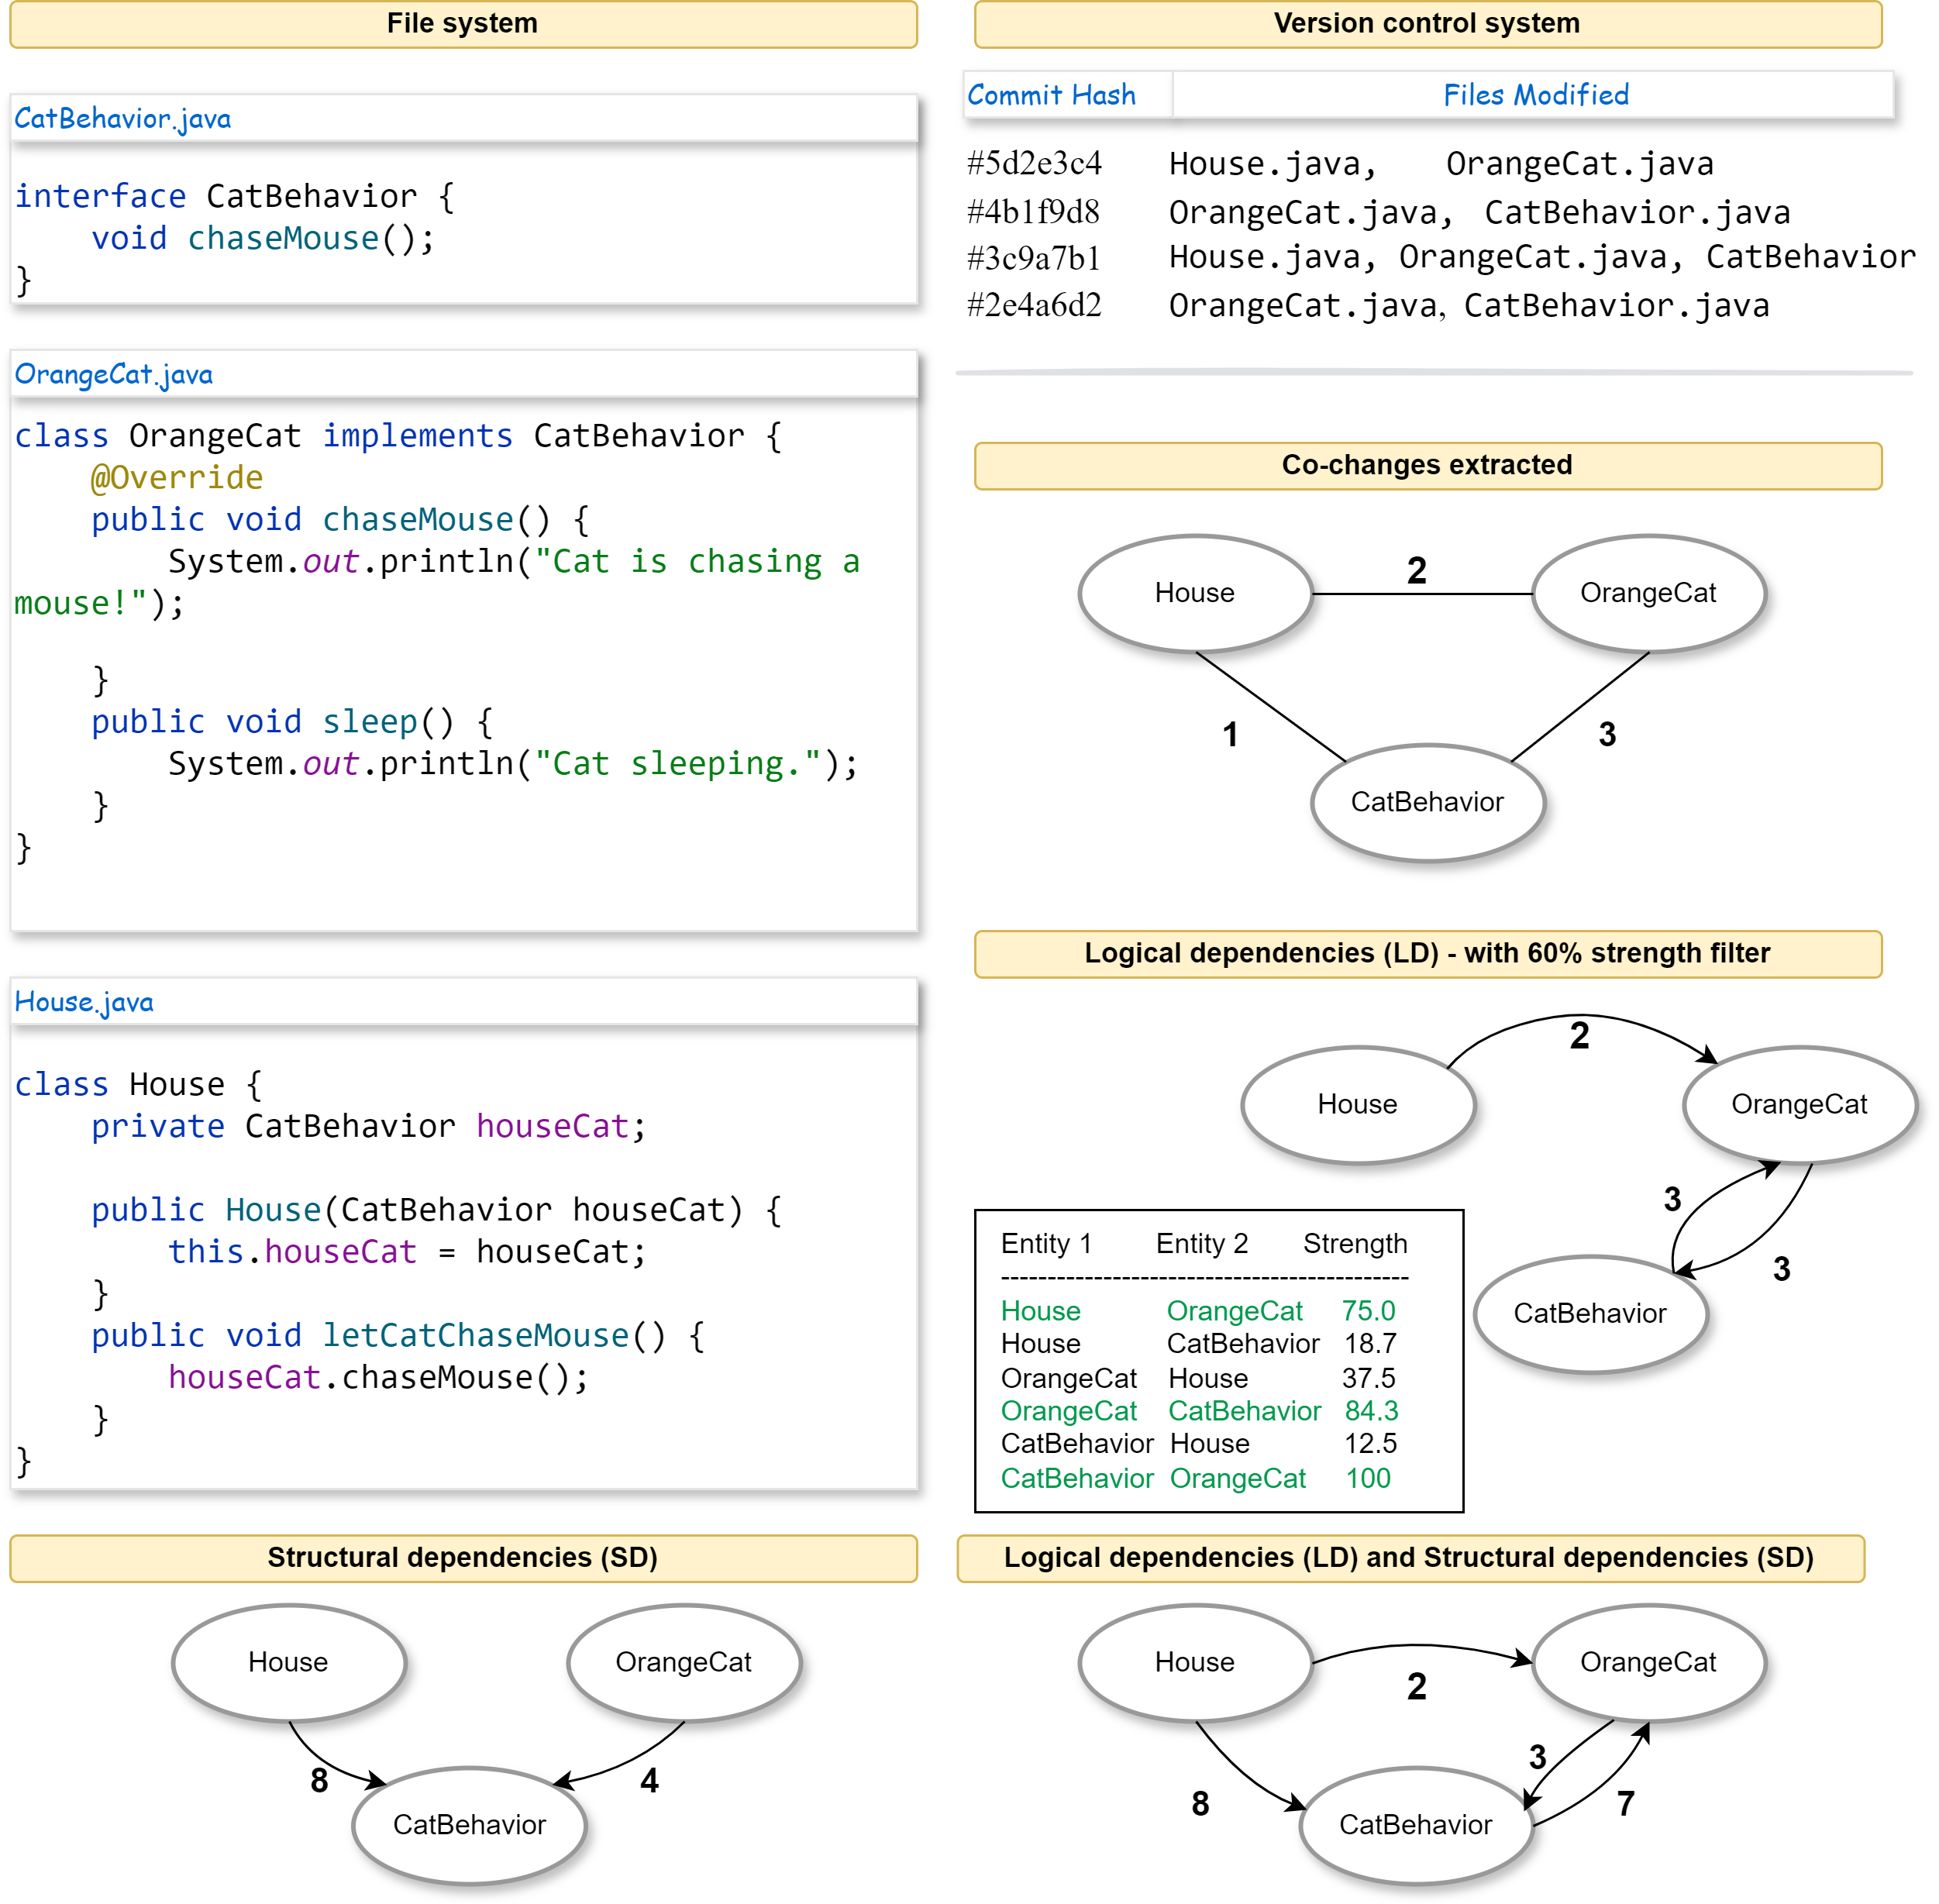
\includegraphics[width=\columnwidth]{codegraph.png}
  \caption{Dependency Graph: Combining structural and logical dependencies.}
  \label{fig:codegraph}
\end{figure}

When structural dependencies (SD) and logical dependencies (LD) are combined in software clustering, both types of relationships are represented within the same graph.

Each entity in the system is represented as a node in the graph, and the dependencies between them are represented as directed weighted edges.

\textit{SD and LD weights are combined} when the same pair of entities appear in both dependencies. In this case, the weights from SD and LD are summed, giving more influence to those entity pairs. When a pair of entities appear only in SD or only in LD, the edge is added to the graph together with its corresponding weight.

Figure \ref{fig:codegraph} illustrates combining structural and logical dependencies in the same dependency graph. The structural dependencies between \texttt{House}, \texttt{OrangeCat}, and \texttt{CatBehavior} entities are visible from the source code analysis.

However, the combination of SD and LD reveals additional insights. One important observation is the logical dependency between \texttt{House} and \texttt{OrangeCat}, which is not observed from the structural analysis. This relation is extracted from version control and filtered using a 60\% strength filter. The strength metric reveals that \texttt{House} and \texttt{OrangeCat} have a significant co-change value of 75.0, usually associated with a strong relationship.

When SD and LD overlap, such as between \texttt{OrangeCat} and \texttt{CatBehavior}, their weights are summed. This summation increases the weight of the dependency, making it more important in the dependency graph.




New structure:
\begin{verbatim}


Chapter 4: Combining structural and logical dependencies
    4.1 Analysis of dependency overlaps
        4.1.1 Measurements of overlaps
        4.1.2 Implications of overlaps
    4.2 Weight assignment
        4.2.1 Structural dependencies weights
        4.2.2 Logical dependencies weights
    4.3 Integration techniques
        4.3.1 Methods for combining dependencies
        4.3.2 Combination framework
\end{verbatim}